\documentclass[../03-Architecture.tex]{subfiles}
\begin{document}

\section{Platener Is Implemented In {\convertify}}
\label{sec:application-platener}

 % - Section overview
 % - Application is built with Convertify (integration with lifecycle events
 %   and rendering engine)
 % - needs-figure :: Application is separated into Packages
 % - Plugins provide scene feature
 % - Client Code to integrate plugins, system and user interfaces

{\platener} is a web-application, that converts 3D-printable
models into laser-cuttable equivalents. This section
describes the implementation of {\platener} within the
{\convertify} framework. Therefore, {\platener} integrates
with the system events and rendering engine of
{\convertify}. As proposed in the preceding section, it uses
several \class{Plugins} to bring its features to the WebGL
scene. Section~\ref{sec:platener-uses-plugins} describes
these plugins briefly.
Section~\ref{sec:platener-pipeline-plugin} shows
architectural details to the most important \class{Plugin}:
the \name{PlatenerPipeline} plugin. This \class{Plugin}
implements different conversion strategies for
{\threedmodel}s. In Section~\ref{sec:client-to-application}
we explain how the application combines user interfaces with
the \class{Dispatcher} and the \class{Plugins}.

\subsection{Platener Uses Plugins to Implement Its Features}
\label{sec:platener-uses-plugins}

The \class{Plugins} composed into {\platener} provide its
computation logic and WebgGL scene rendering. We will give a
brief introduction of each plugin in the following
paragraphs.

\subsubsection{Platener Pipeline Plugin}

The \name{PlatenerPipeline} plugin does the major work on
converting {\threedmodels} to 2D-plates. The plugin defines
multiple conversion approaches. A conversion is an
approximation of the original model with plates.
Figure~\ref{fig:conversion:plate} and
Figure~\ref{fig:conversion:stacked} show two conversion
results. This plugin generates a set of 2D-paths, so that
the conversion can be produced with a {\lasercutter}. The
paths are depicted in Figure~\ref{fig:conversion:paths}.
Section~\ref{sec:platener-pipeline-plugin} explains the
architecture of the \name{PlatenerPipeline} plugin in
detail.

\begin{figure}[h]
  \centering
  \begin{subfigure}[a]{0.3222\textwidth}
    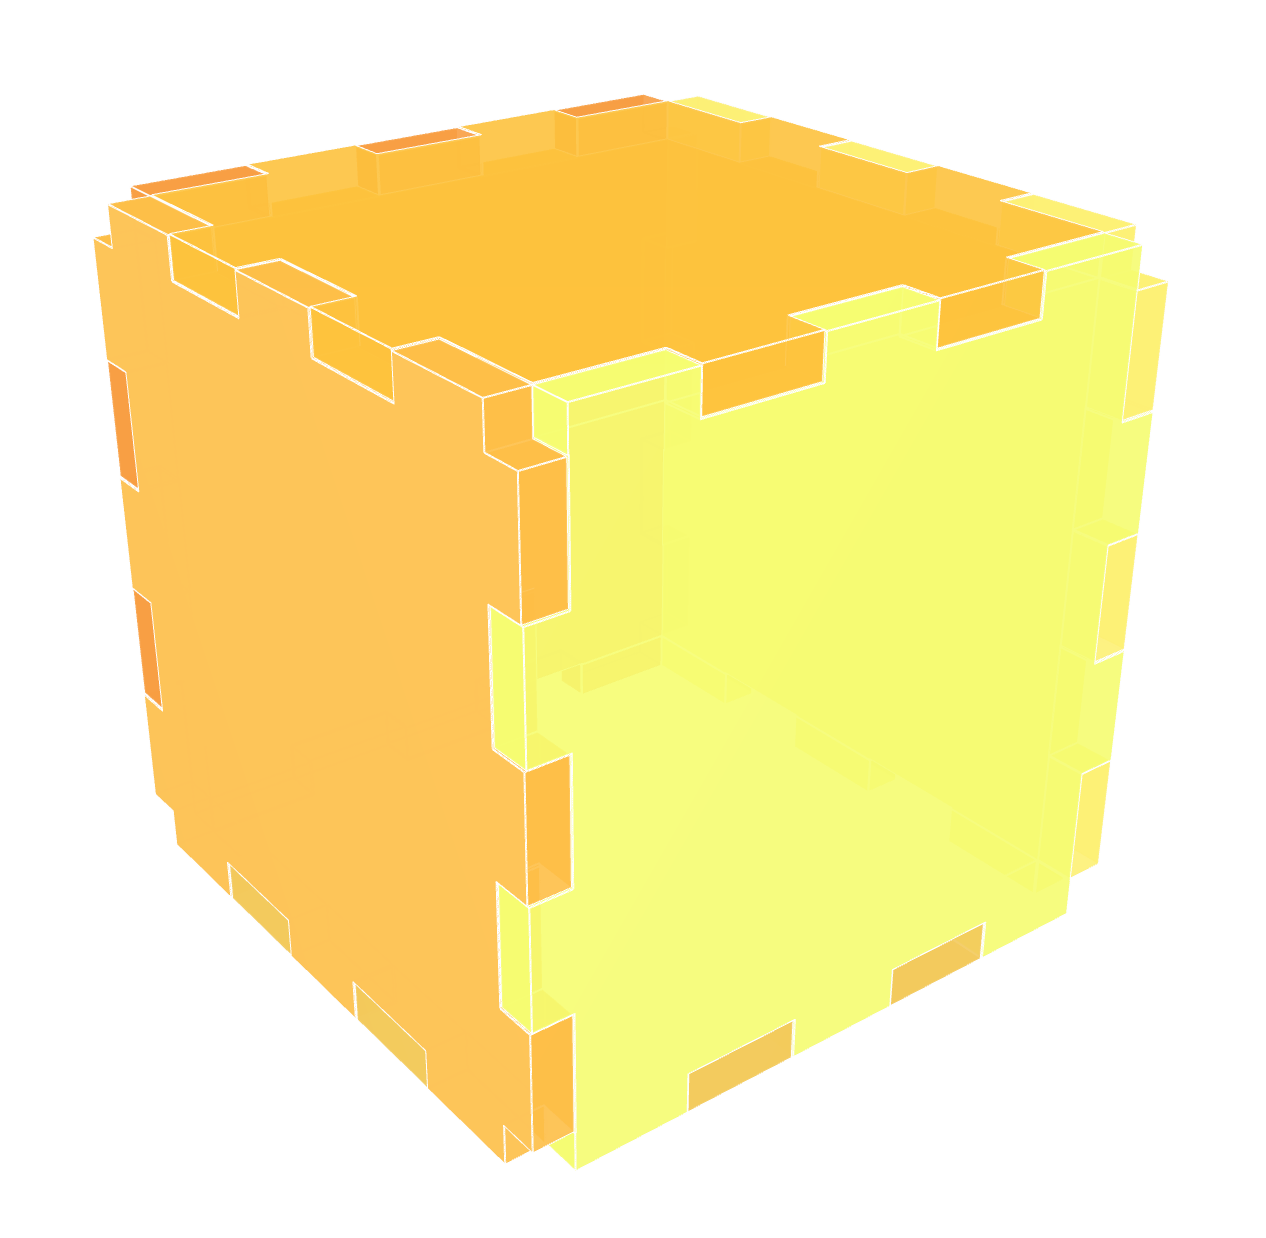
\includegraphics[width=\textwidth]{03-architecture-box-hull}
    \caption{A box converted with hull approximation.}
    \label{fig:conversion:plate}
  \end{subfigure}
  \begin{subfigure}[b]{0.3222\textwidth}
    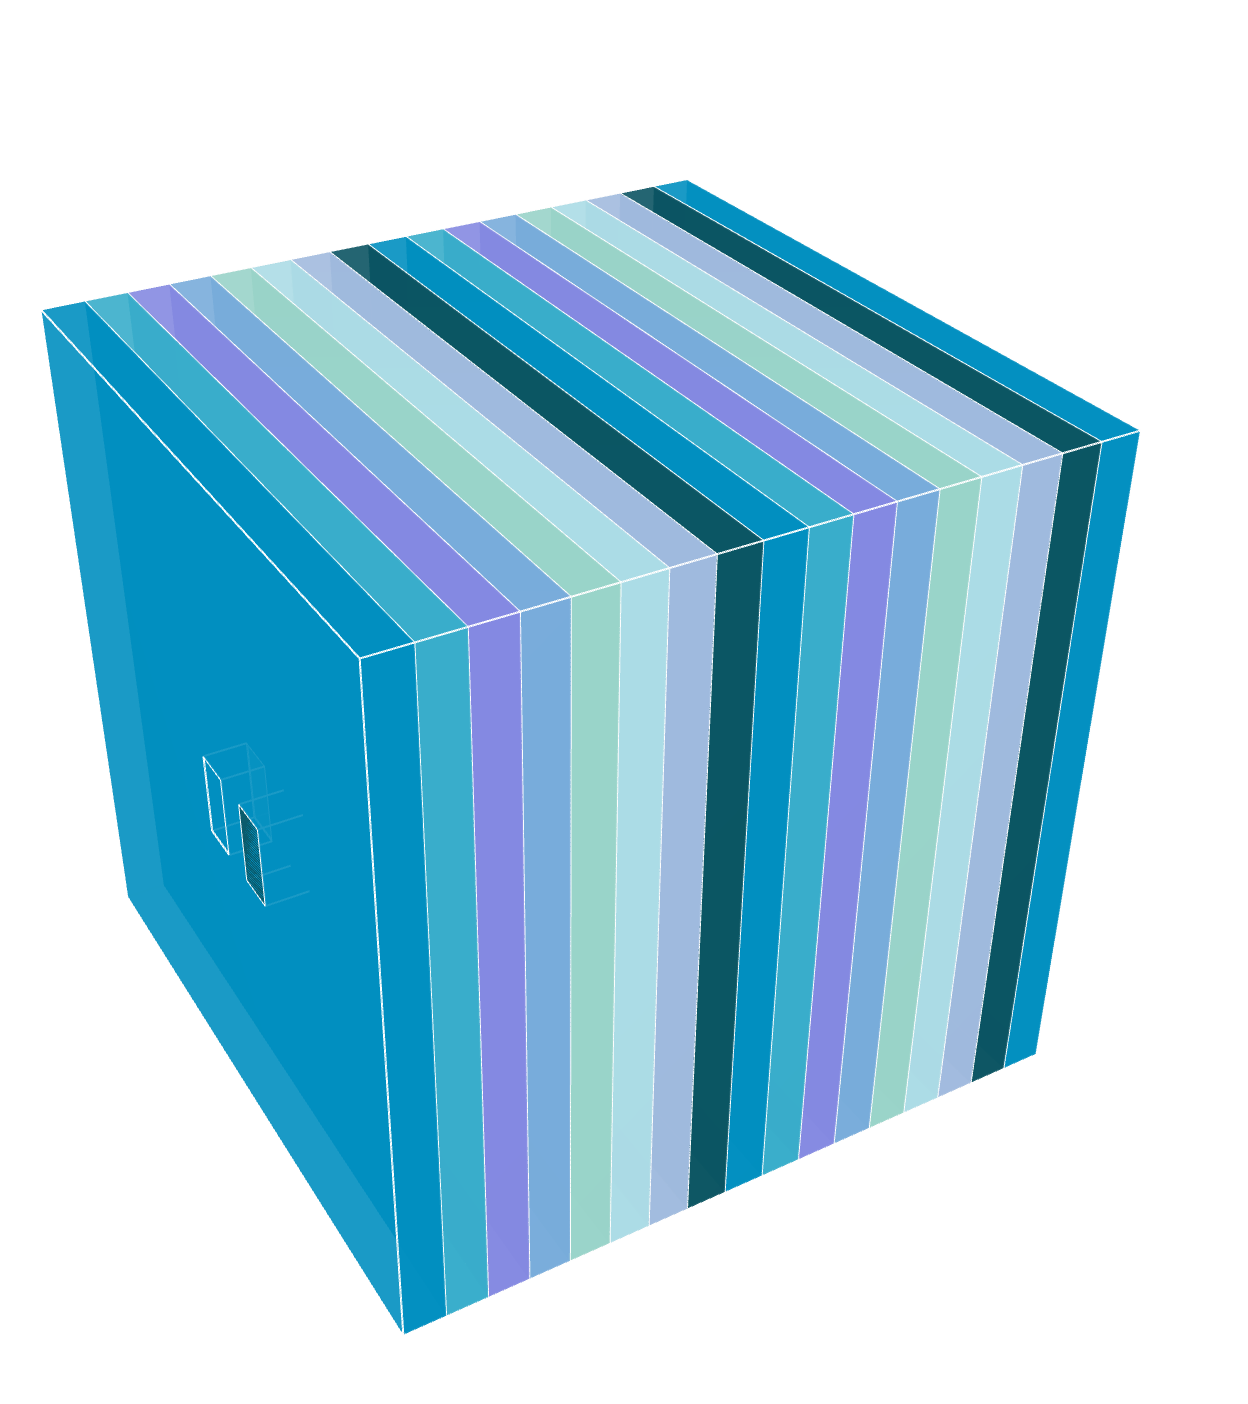
\includegraphics[width=\textwidth]{03-architecture-box-stacked}
    \caption{A box converted with stacked approximation.}
    \label{fig:conversion:stacked}
  \end{subfigure}
  \begin{subfigure}[c]{0.3222\textwidth}
    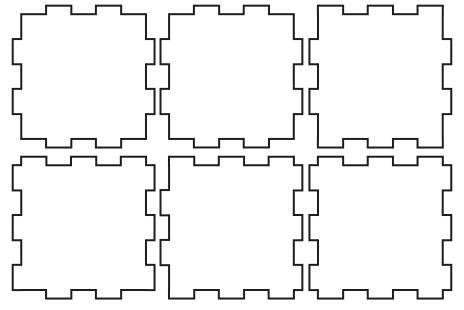
\includegraphics[width=\textwidth]{03-architecture-cutting-plan-box-hull}
    \caption{2D-paths of the box converted with hull approximation.}
    \label{fig:conversion:paths}
  \end{subfigure}
  \caption{Results of the \name{PlatenerPipeline} plugin.}
  \label{fig:conversion}
\end{figure}

% The \name{PlatenerPipeline} plugin is the main computation unit.
% The \class{Plugin} defines multiple {\fabmethod}s. A
% {\fabmethod} is a conversion approach of a \threedmodel.
% Multiple computation steps, which can manipulate the input
% model, are chained after another to produce 2D- or
% 3D-output. For example, construction plans in the format of
% {\svgfile}s are such an output, see Figure~\ref{}
% \note{construction plans figure}.
% Section~\ref{sec:platener-pipeline-plugin} explains the
% architecture of the \name{PlatenerPipeline} plugin in detail.

\subsubsection{Node Visualizer Plugin}

We visualize the results of the \name{PlatenerPipeline}
plugin in the WebGL view. The \name{NodeVisualizer} plugin
renders the results of each conversion and its intermediate
computation steps respectively. With the help of this we
debug the results of the computation visually. As explained
in Section~\ref{}\note{section walkthrough}, we select a
single visualization at a time to inspect the results of the
step associated with the visualization.
Figure~\ref{fig:steps:plate} shows a head-mounted display in
the \name{Plate} step. Figure~\ref{fig:steps:ui} shows the
selection of that visualization in the user interface.

\begin{figure}[h]
  \centering
  \begin{subfigure}[a]{0.48\textwidth}
    \includegraphics[width=\textwidth]{}
    \caption{A head-mounted display, consisting of plates only.}
    \label{fig:steps:plate}
  \end{subfigure}
  \begin{subfigure}[b]{0.48\textwidth}
    \includegraphics[width=\textwidth]{}
    \caption{The selection of the intermediate plate step in
      the user interface.}
    \label{fig:steps:ui}
  \end{subfigure}
  \label{fig:steps}
  \caption{Visual debugging of intermediate conversion results.}
\end{figure}

\subsubsection{Scorer Plugin}

We run multiple conversion approaches sequentially. Then, we choose
the best fitted conversion as output. Thus each conversion
is scored by a scoring algorithm. This
\clas{Plugin} provides such scoring algorithms.

\subsubsection{Solution Selection Plugin}

This plugin utilizes the \name{Platener Pipeline} plugin and
the \name{Scorer} plugin to run and evaluate all conversion
approaches. It outputs the result of the conversion with the
best score.

\subsubsection{Coordinate System Plugin}

This plugin provides orientation enhancements for the WebGL
scene. Rendering xyz-axes and a an axis-aligned grid, users
can grasp alignment and dimensions of {\threedmodel}s.
Figure \ref{fig:architecture_overview_coordinate_system}
shows the coordinate system in the WebGL view. The
Coordinate System is taken from \emph{Brickify} as
is\cite{}\note{ref chapter in brickify}.

\begin{figure}
  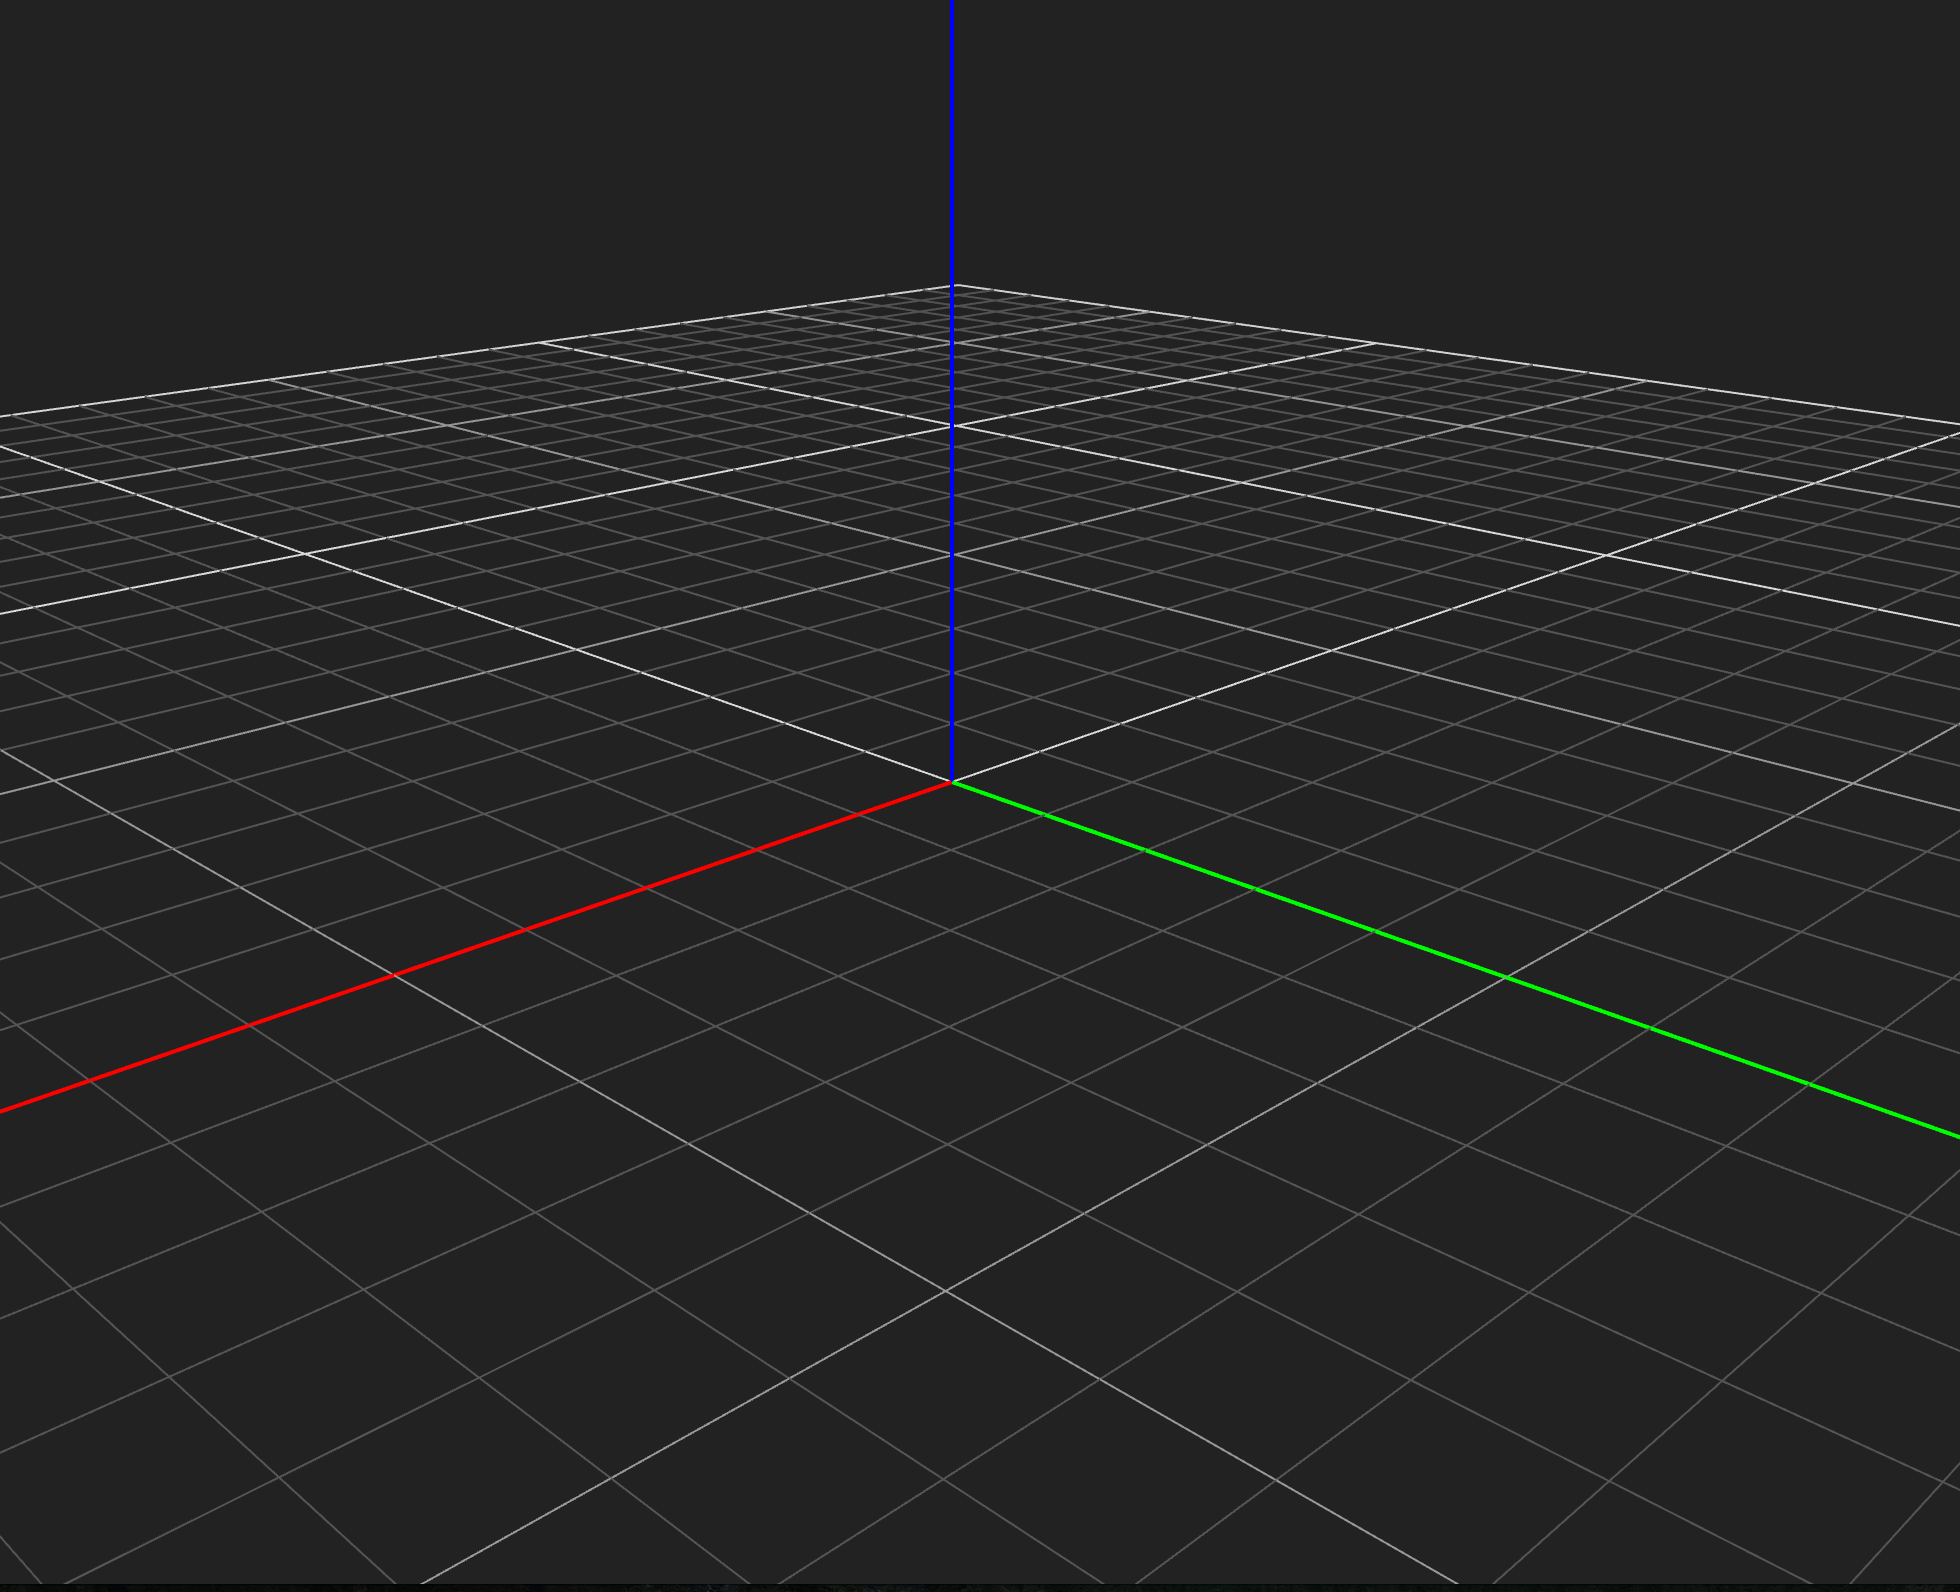
\includegraphics[width=1\columnwidth]{03-architecture_overview_coordinate_system}
  \caption{An empty scene showing the coordinate system.}
  \label{fig:architecture_overview_coordinate_system}
\end{figure}

\subsubsection{Isolated Testing Plugin}

While we developed on different stages of a sequentially
executed conversion approach in parallel, we needed a
mechanism to test each component of the conversion before
its preceeding or succeeding components were completely
implemented. The \name{IsolatedTesting} plugin provides an
isolated environment, which allows to execute a single
intermediate computation step of a conversion approach with
pre-defined input.

\subsection{The PlatenerPipeline Plugin Computes the Model
  Conversions}
\label{sec:platener-pipeline-plugin}

% - Subsection overview

The \name{PlatenerPipeline} is the main computation unit of
{\platener}. It contains algorithms and data structures to
bring the {\threedmodel} into a 2D-representation suitable
for a {\lasercutter}. In this section we dive into details
about the computation process. First we look at
{\platener}'s three conversion approaches. Then, we explain
the composition of conversion approaches from computation
steps into a \class{Pipeline} data structure. Finally, we
present the \class{PipelineState}, a data structure which
allows to take a snapshot of the computation state in
between two computation steps. The \class{PipelineState} is
used to render the visualizations of the
\name{NodeVisualizer} plugin.

% - needs-figure :: Pipelining Approach to subdivide the problem space
% - PipelineSteps as single computation units
% - Several Pipeline Steps make up a Fabrication Method

\subsubsection{{\platener} Presents Three Conversion
  Approaches}

The \name{PlatenerPipeline} plugin facilitates conversion
approaches. We call such a conversion approach
\class{\fabmethod}.
%A {\fabmethod} is a conversion approach of a {\threedmodel}.
It defines a linear process of analyzing a {\threedmodel}
and thereby creates a suitable equivalent of the model,
consisting of plates only. A \class{\fabrication} method
divides the conversion problem into smaller problems. Thus,
it provides a set of algorithms, which are executed
sequentially. Each algorithm solves a single subproblem. The
algorithms work on results of previously executed
algorithms. We refer to a sequence of algorithms as
\class{Pipeline}. Each algorithm in the \class{Pipeline} is
an intermediate computation step, called
\class{PipelineStep}. The first \class{PipelineStep} works
on the face-vertex-mesh of the model. The last
\class{PipelineStep} returns a directly exportable data
format, in our case a {\zipfile} containing the
2D-construction plans. The composition of
\clas{PipelineSteps} into a \class{Pipeline} is shown in
Figure~\ref{fig:pipeline-from-steps}. \class{PipelineSteps}
are independent from the \class{\fabmethod} and thus, can be
shared between different \class{{\fabmethod}s}. {\platener}
provides three \class{{\fabmethod}s}. The following paragraphs
present each method briefly.

\begin{figure}[h]
\centering
\begin{verbatim}
- show multiple pipeline steps with inlets/ outlets of
pipeline state
- make clear, that a pipeline step is an algorithm, solving
a sub problem
- pipeline like a swimming lane, where pipeline steps
connect
- a model comes in
- a construction plan falls out (zip file)
\end{verbatim}
\caption{A \class{Pipeline} is composed from
  \class{PipelineSteps}}
\label{fig:pipeline-from-steps}
\end{figure}

\paragraph{Plate Method}

This \class{\fabmethod} does hull and surface
reconstructions of the input model. We produce a set of
plates which are connected via finger joints to approximate
the original {\threedmodel}. Therefore, we first detect the
outlines of all surfaces in the model. Then, we search for
existing plates based on that surfaces. For example two
parallel surfaces form an \name{inherent} plate, when they
are about three to five millimeters apart. After we found
all \name{inherent} plates, we construct plates from the
remaining surfaces by \name{extruding} the planar shapes.
Then we connect the plates with finger joints where they
touch each other. Figure~\ref{fig:model-fingers} shows
plates connected with finger joints.
Figure~\ref{fig:overview-plate-steps} depicts the important
\class{PipelineSteps} of the \name{Plate Method}.
\note{remake this figure with our steps}

\begin{figure}[h]
  \centering
  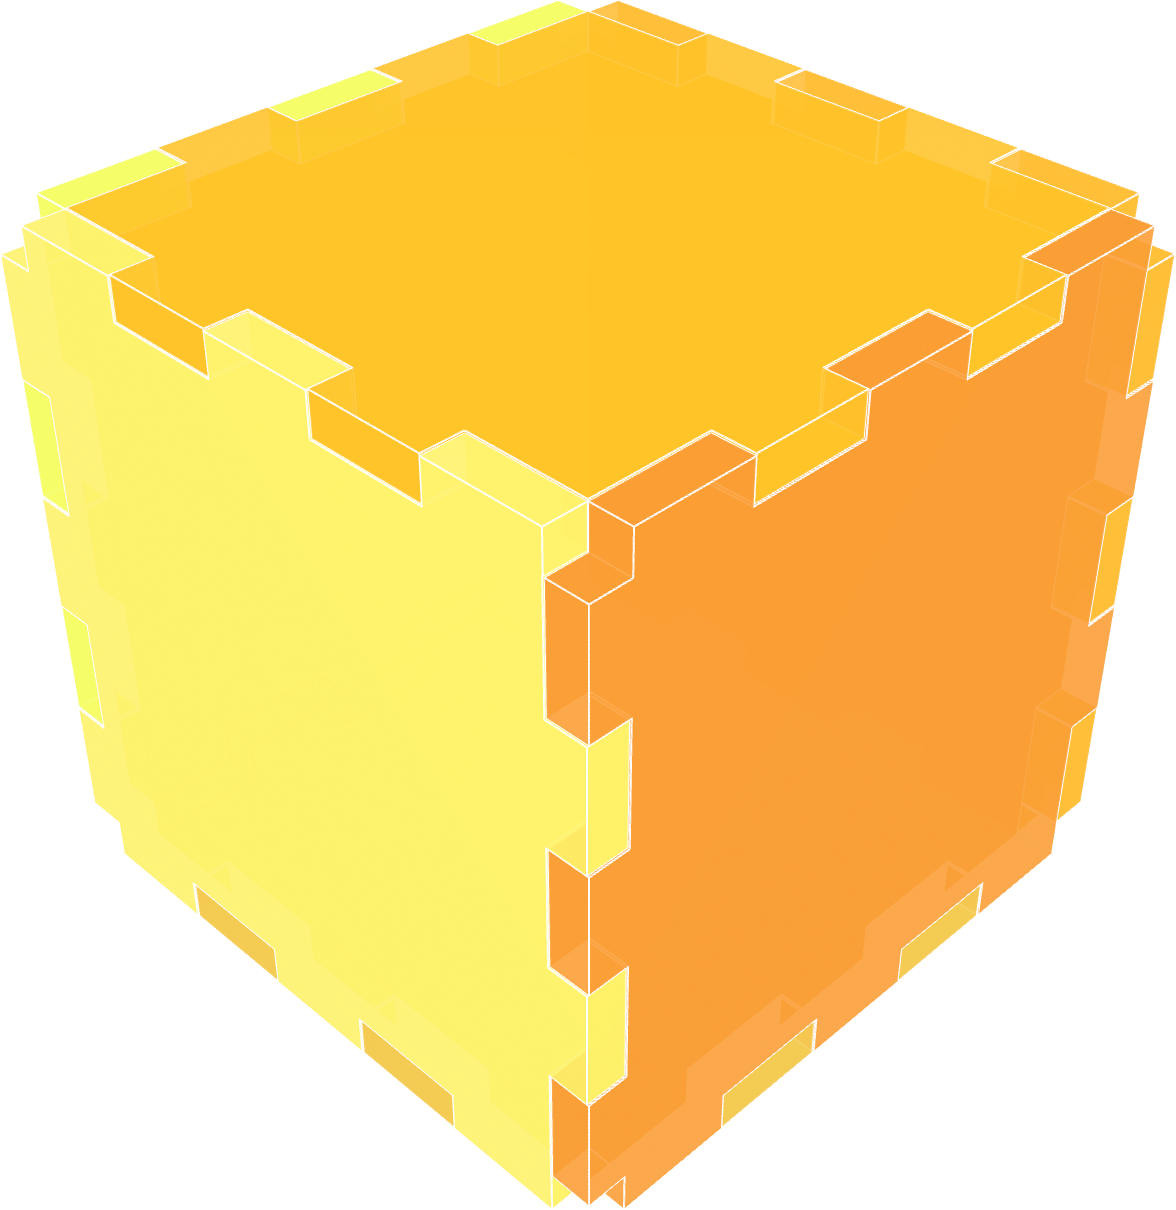
\includegraphics[width=0.6\textwidth]{03-architecture-box-fingers}
  \caption{A model built from plates, connected with finger
    joints.}
  \label{fig:model-fingers}
\end{figure}

\begin{figure}[h]
  \centering
  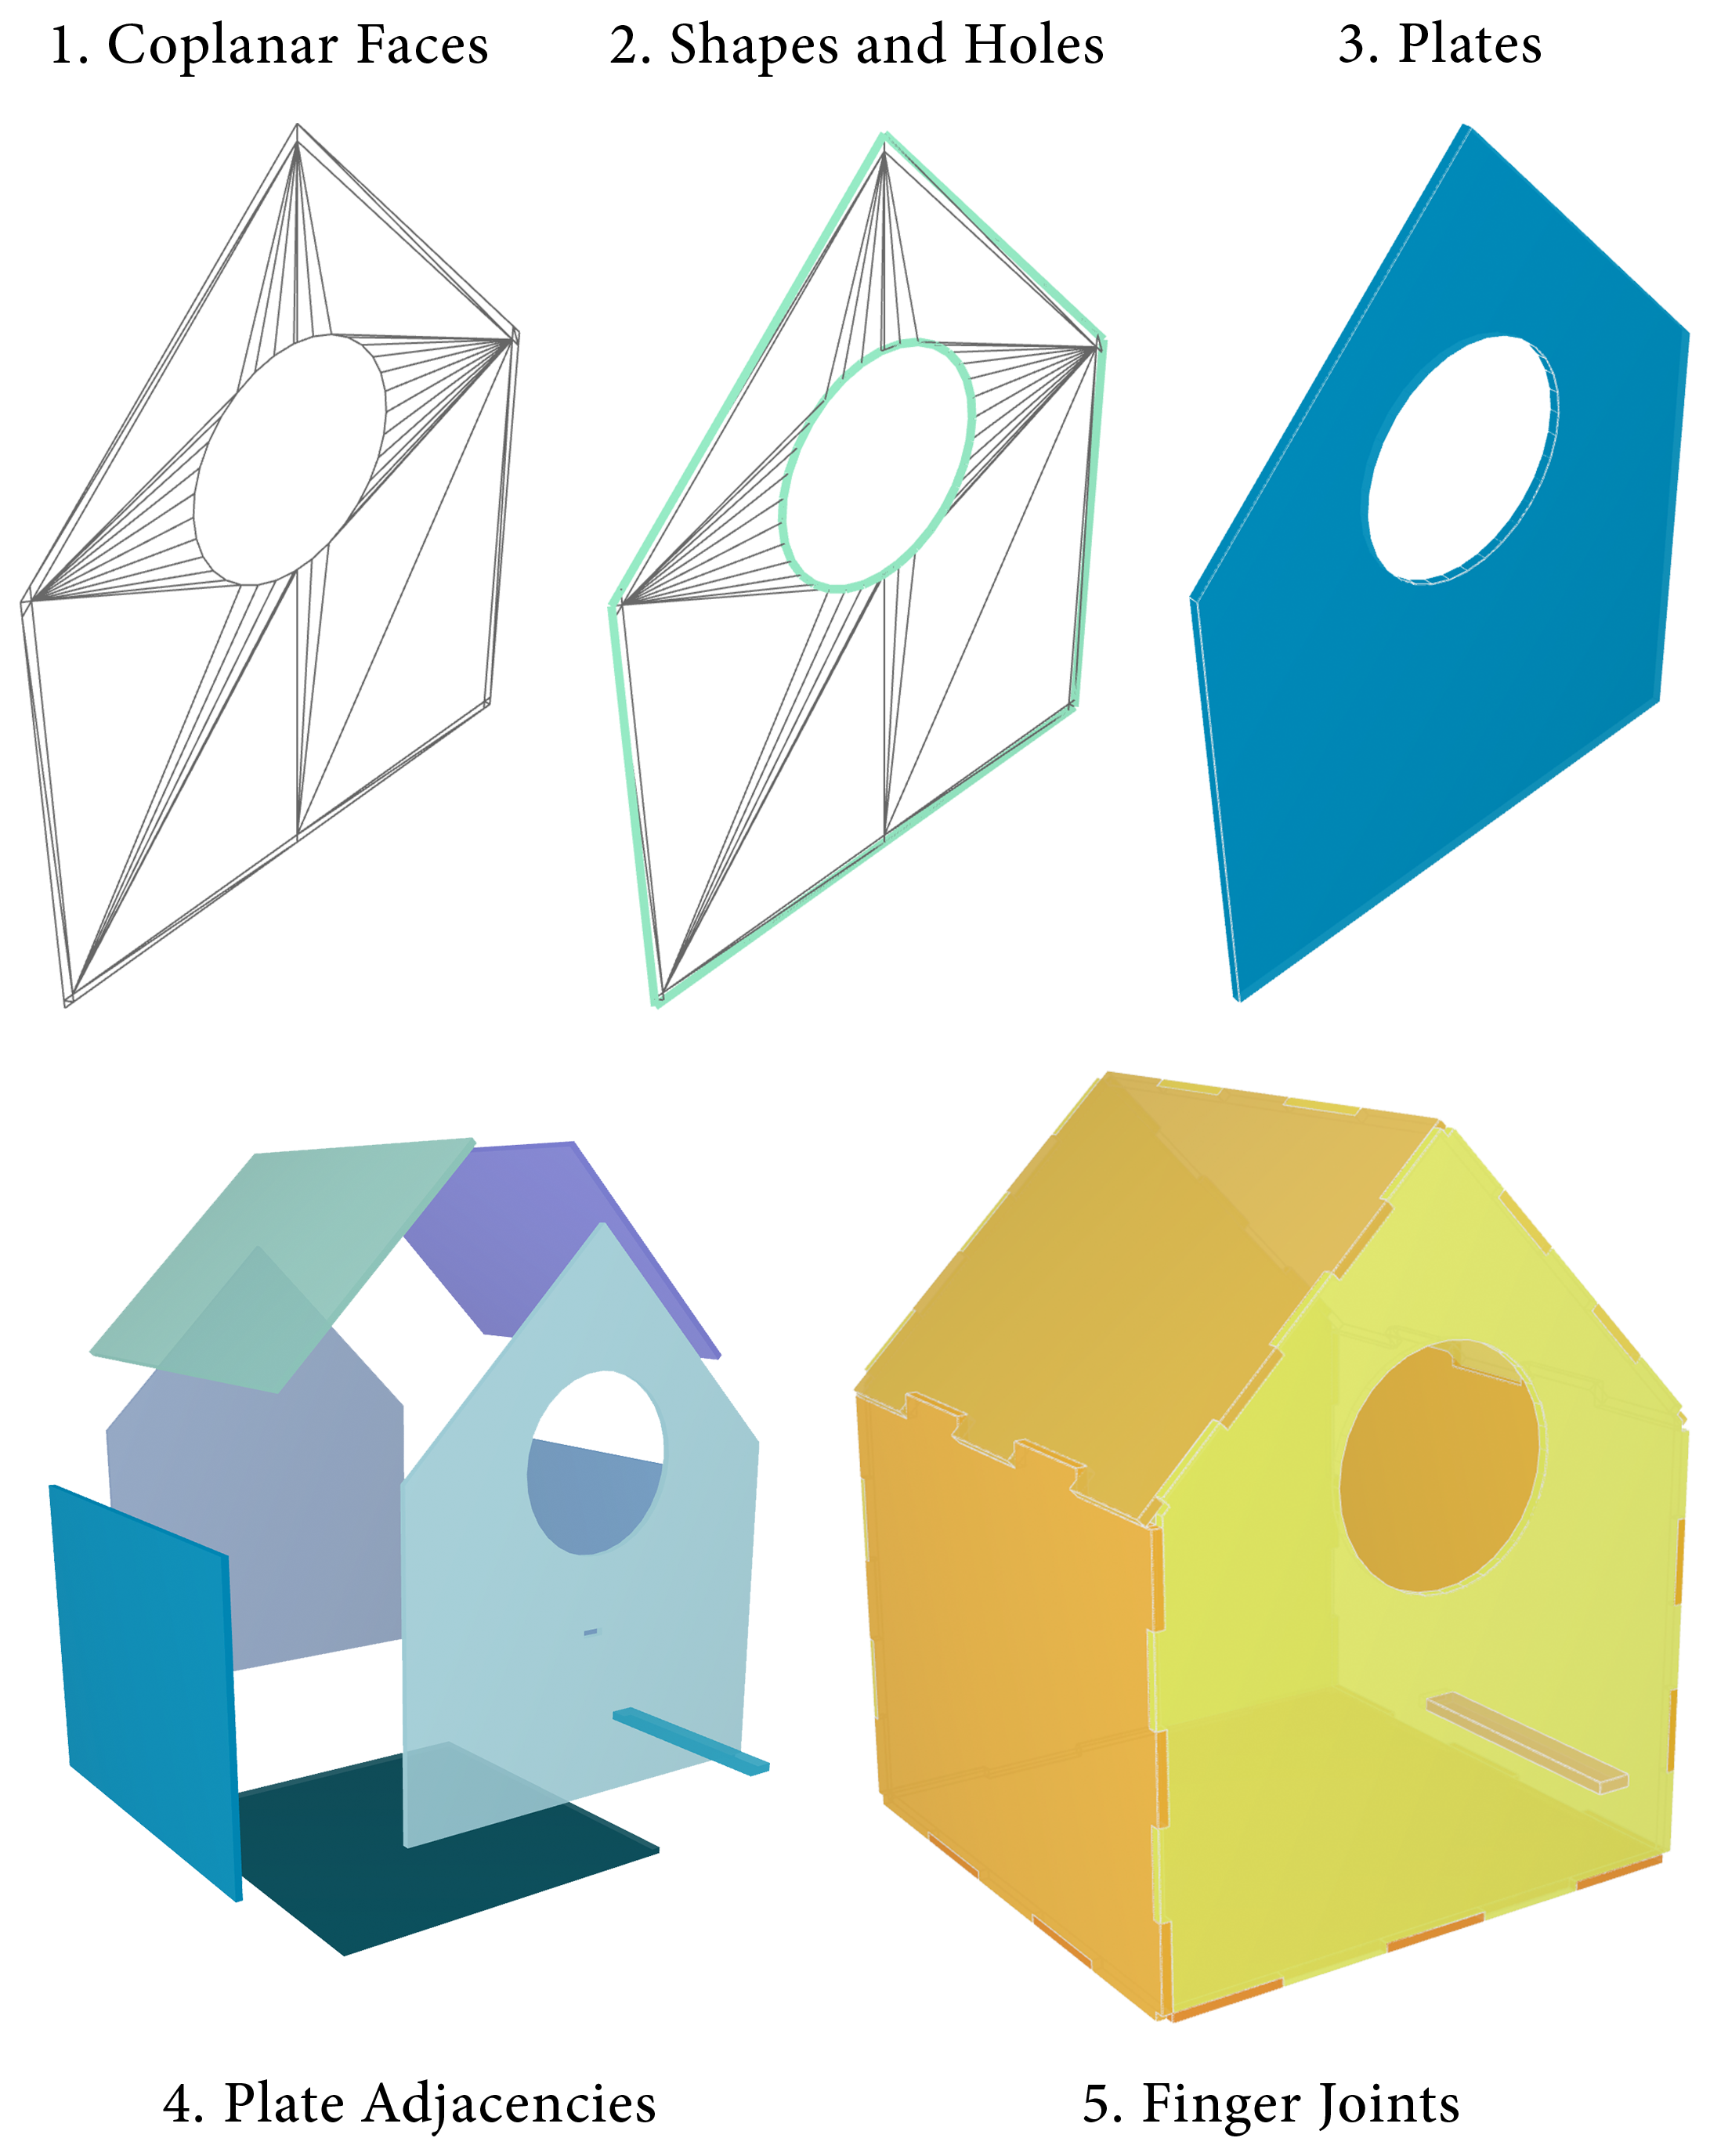
\includegraphics[width=1\textwidth]{03-architecture-pipeline-steps-overview}
  \caption{An overview of computation steps that are applied
    to the model, so that it can be built from plates..}
  \label{fig:overview-plate-steps}
\end{figure}


\note{ref to chapters which explain the algorithms to that
  method in detail}

\paragraph{Stacked Plates Method}

This \class{\fabmethod} does volume reconstructions of the
input model. We stack plates onto each other to approximate
the shape of the original model, see
Figure~\ref{fig:stacked-rabbit}. This preserves the look and
feel of the model. We slice the model into equally thick
layers, which form the plates. The plates are then connected
via shafts to simplify the assembly process.

\begin{figure}[h]
  \centering
  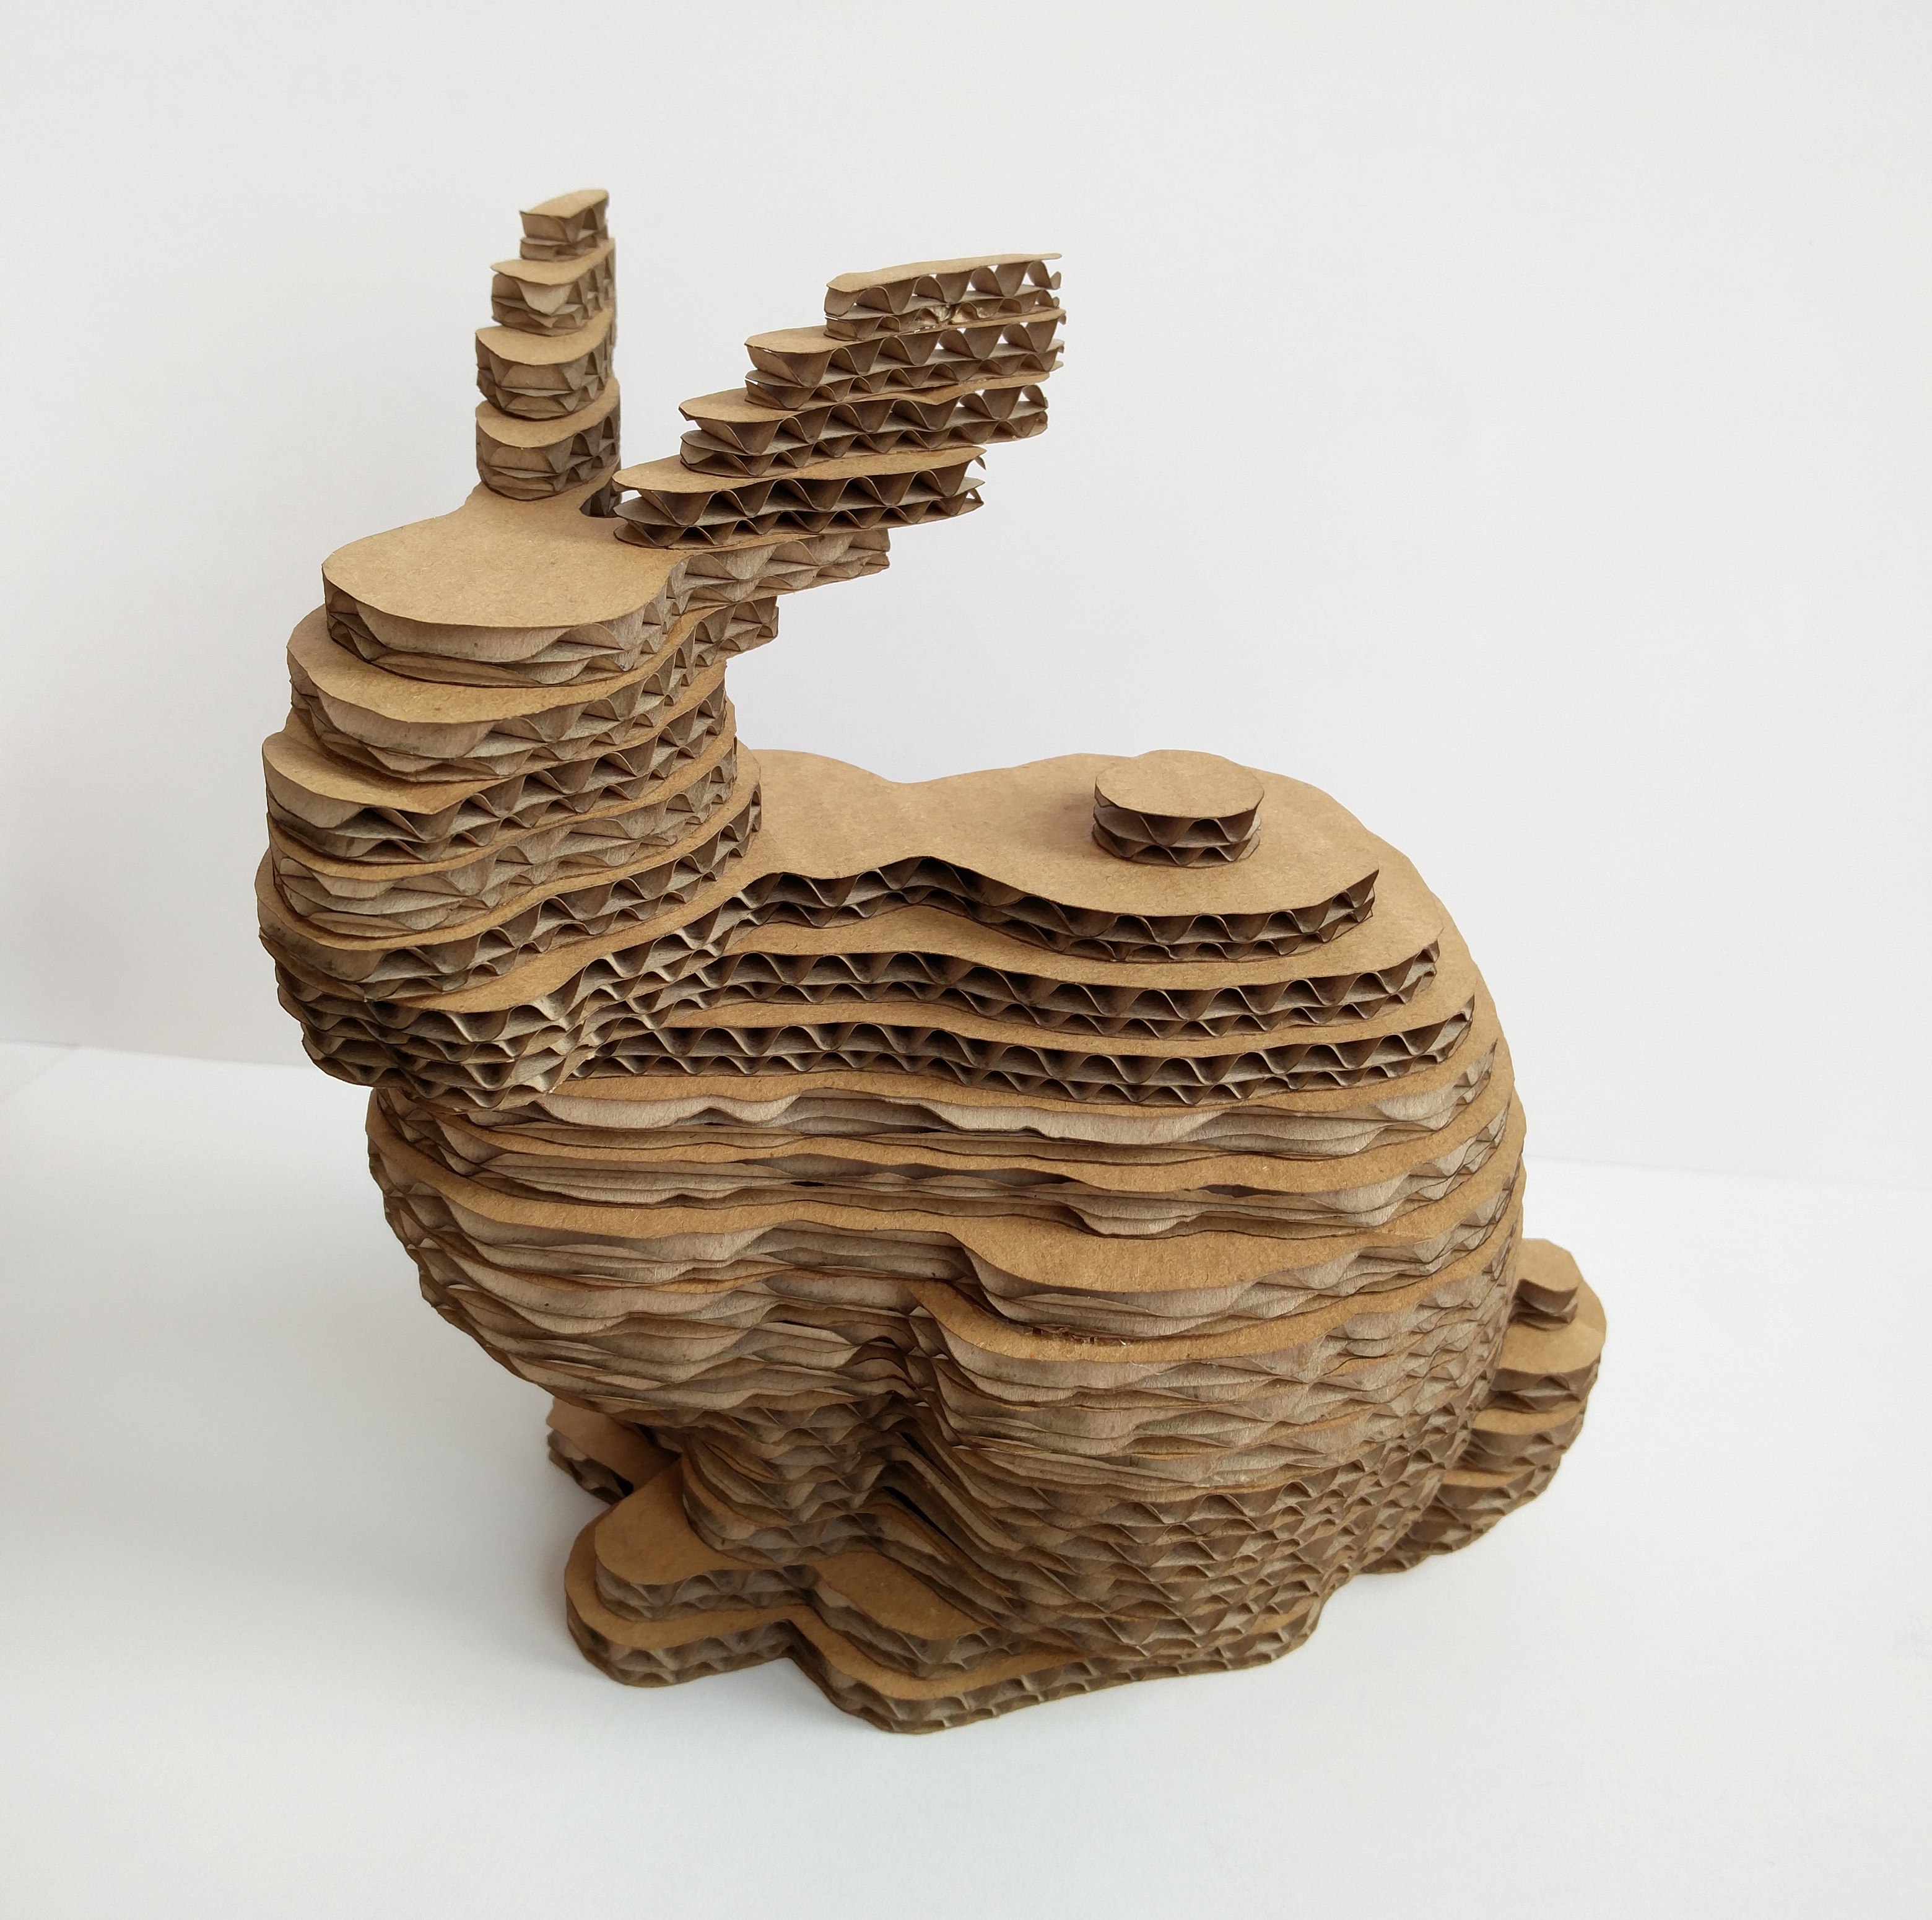
\includegraphics[width=0.6\textwidth]{03-architecture-rabbit-stacked}
  \caption{A rabbit model converted to plates with
    stacking.}
  \label{fig:stacked-rabbit}
\end{figure}
\note{ref to chapters which explain the algorithms to that
  method in detail}

\paragraph{Classifier Method}

This is an advanced conversion approach, combining intense
mesh analysis and sophisticated construction techniques of
known geometries. This \class{\fabmethod} will be more
robust when converting models with noisy mesh data, e.g
{\threedmodel}s with lots of texture on their surface. We
analyze the model for primitive geometries using random
algorithms. Primitive geometries are planes, prisms, boxes,
cylinders or spheres. The model is structured into an
hierarchical graph structure, similar to a scene graph,
consisting of these primitive geometries only. For each of
these primitives we know a conversion approach to plates,
which will then give better results for the conversion of
the whole input model. The \name{Classifier Method} is a
proposal and still work in progress. We can currently
classify a subset of the primitive geometries.
Figure~\ref{fig:tiki-cylinder} shows the classification of a
cylinder in a model. In Chapter~\ref{} \note{ref the
  chapter!} we give details about the random algorithm,
which classifies the primitives.

\begin{figure}[h]
  \centering
  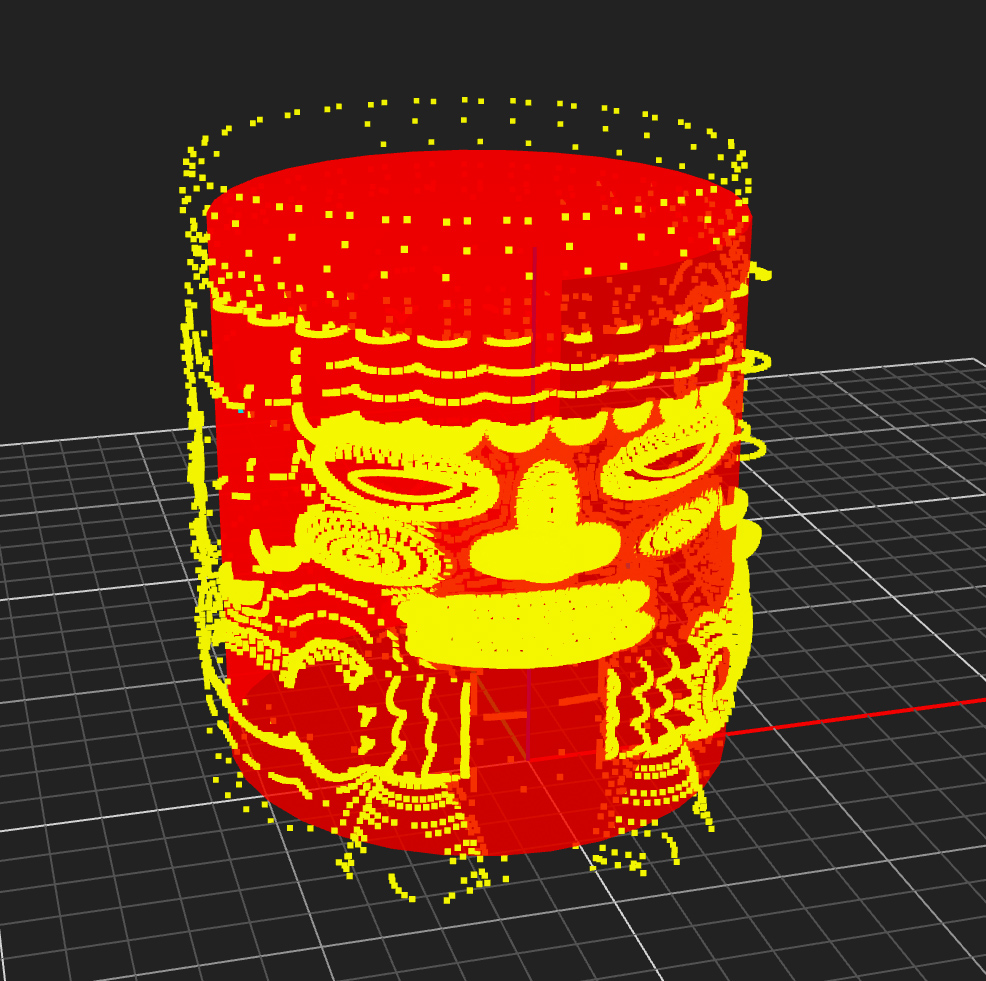
\includegraphics[width=0.6\textwidth]{03-architecture-tiki-cylinder}
  \caption{A classified cylinder in a model with textures.
    The yellow points, show the outline of the actual model.}
  \label{fig:tiki-cylinder}
\end{figure}

\paragraph{}

\note{summary}

\subsubsection{Pipeline Steps Compute Cloneable State}

Each \class{\fabmethod} assembles a \class{Pipeline} from
\class{PipelineSteps}. \class{PipelineSteps} work on the
data of previous computation steps and pass the data to the
next compution steps. To improve the development and
debugging experience, we not only pass the results of the
\class{PipelineStep} to the following step, but we also
preserve a snapshot of the data. We call the state of a
given data structure at a given point in time a snapshot. A
snapshot of the computed data is used to render a visual
representation of the data. The visual representation gives
a clear understanding of the data and thus enhances the
development and debugging experience. In this section we
explain how the \class{Pipeline} takes snapsots of the
results of \class{PipelineSteps}. Note, that the
\class{PipelineSteps} are merely computation units. All
visual output is done in the \name{NodeVisualizer} plugin.

When we take a snapshot of the results of a
\class{PipelineStep}, we ensure, that modifications of a
latter \class{PipelineStep} will not alter the data in the
snapshot of a previous \class{PipelineStep}. Otherwise, the
\name{NodeVisualizer} plugin renders corrupted visuals for
the previous step. Figure~\ref{fig:corrupt} shows how the surface
reconstruction step, which comes early in the
\class{Pipeline}, is effected by the creation of finger
joints.

\begin{figure}[h]
  \centering
  \begin{subfigure}[a]{0.3222\textwidth}
    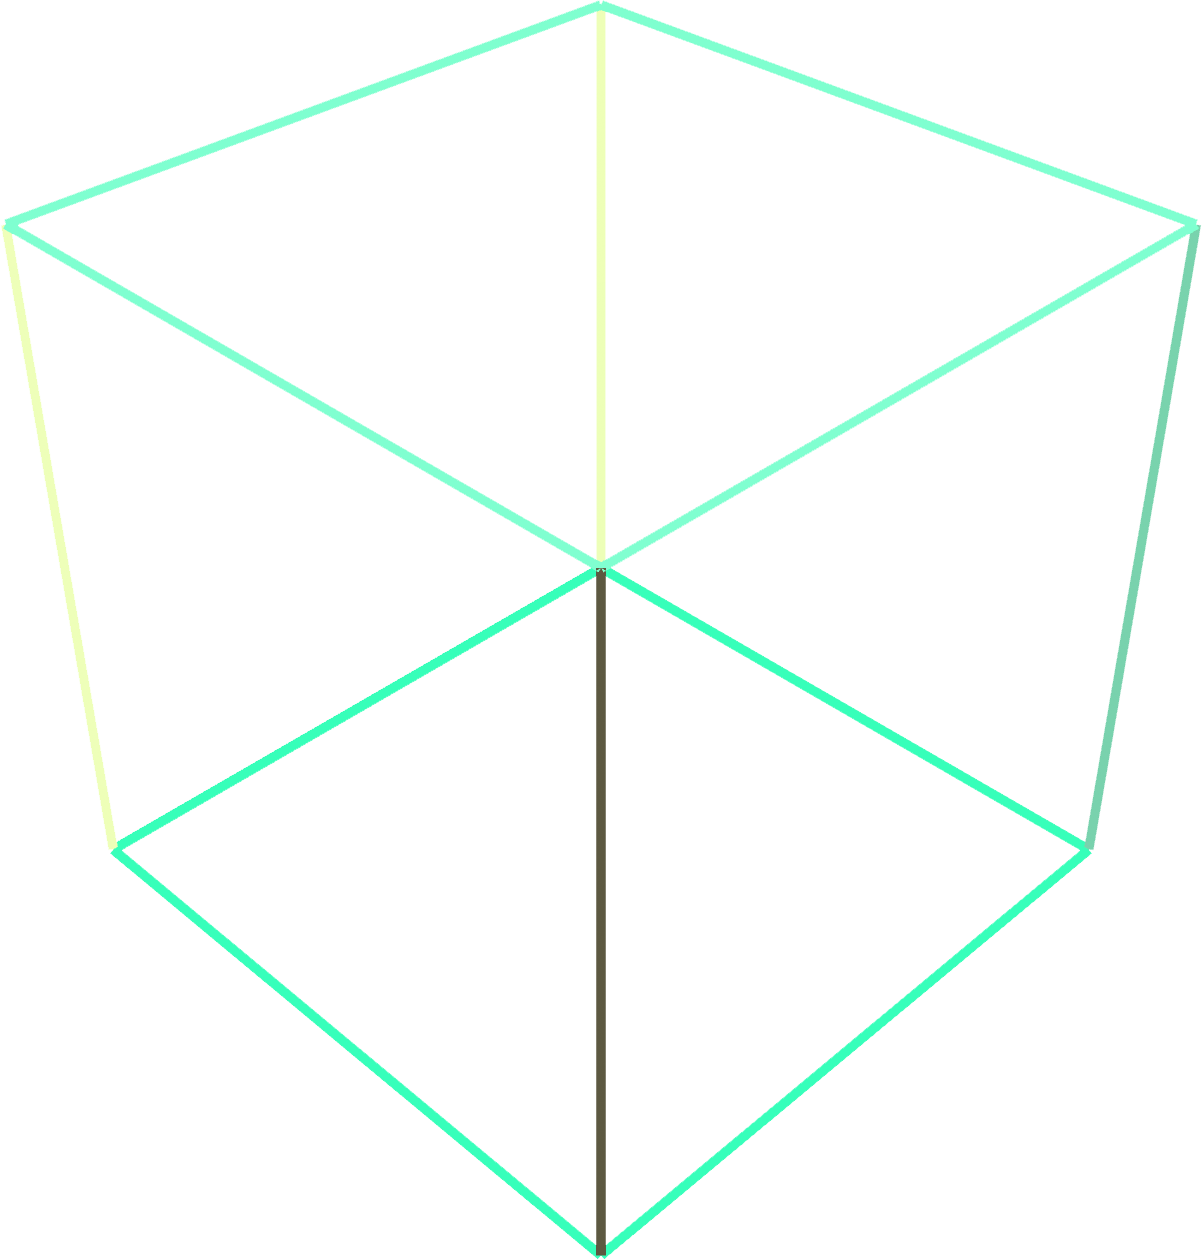
\includegraphics[width=\textwidth]{03-architecture-box-shapes}
    \caption{The shapes of a box.}
    \label{fig:corrupt:shapes}
  \end{subfigure}
  \begin{subfigure}[b]{0.3222\textwidth}
    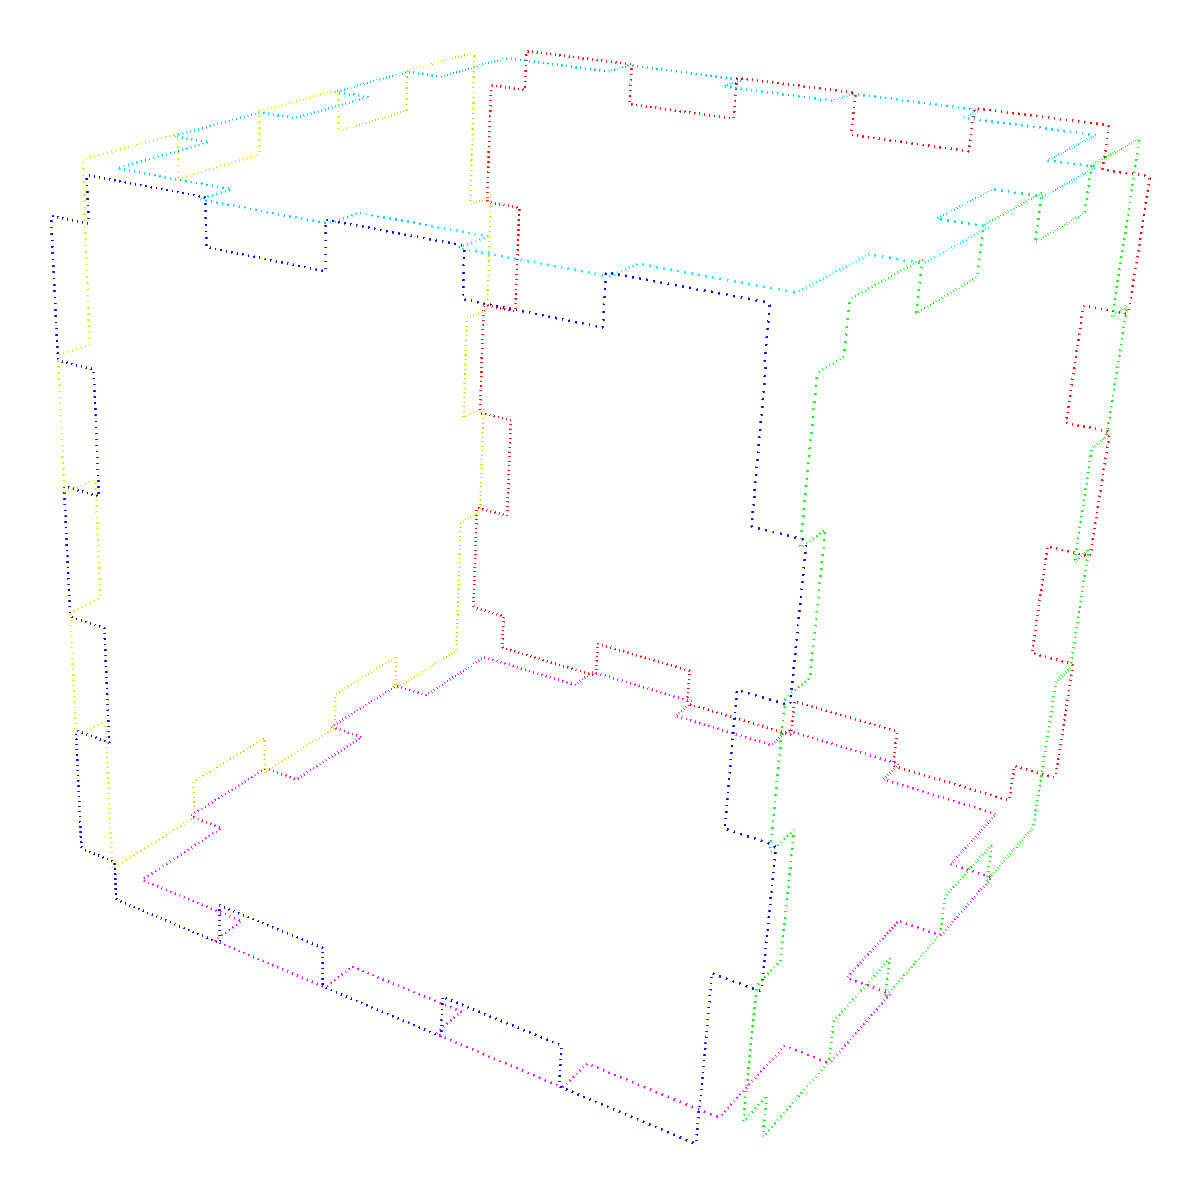
\includegraphics[width=\textwidth]{03-architecture-box-shapes-with-fingers}
    \caption{Corrupted shapes of a box, showing the finger joints.}
    \label{fig:corrupt:shapes-fingers}
  \end{subfigure}
  \begin{subfigure}[c]{0.3222\textwidth}
    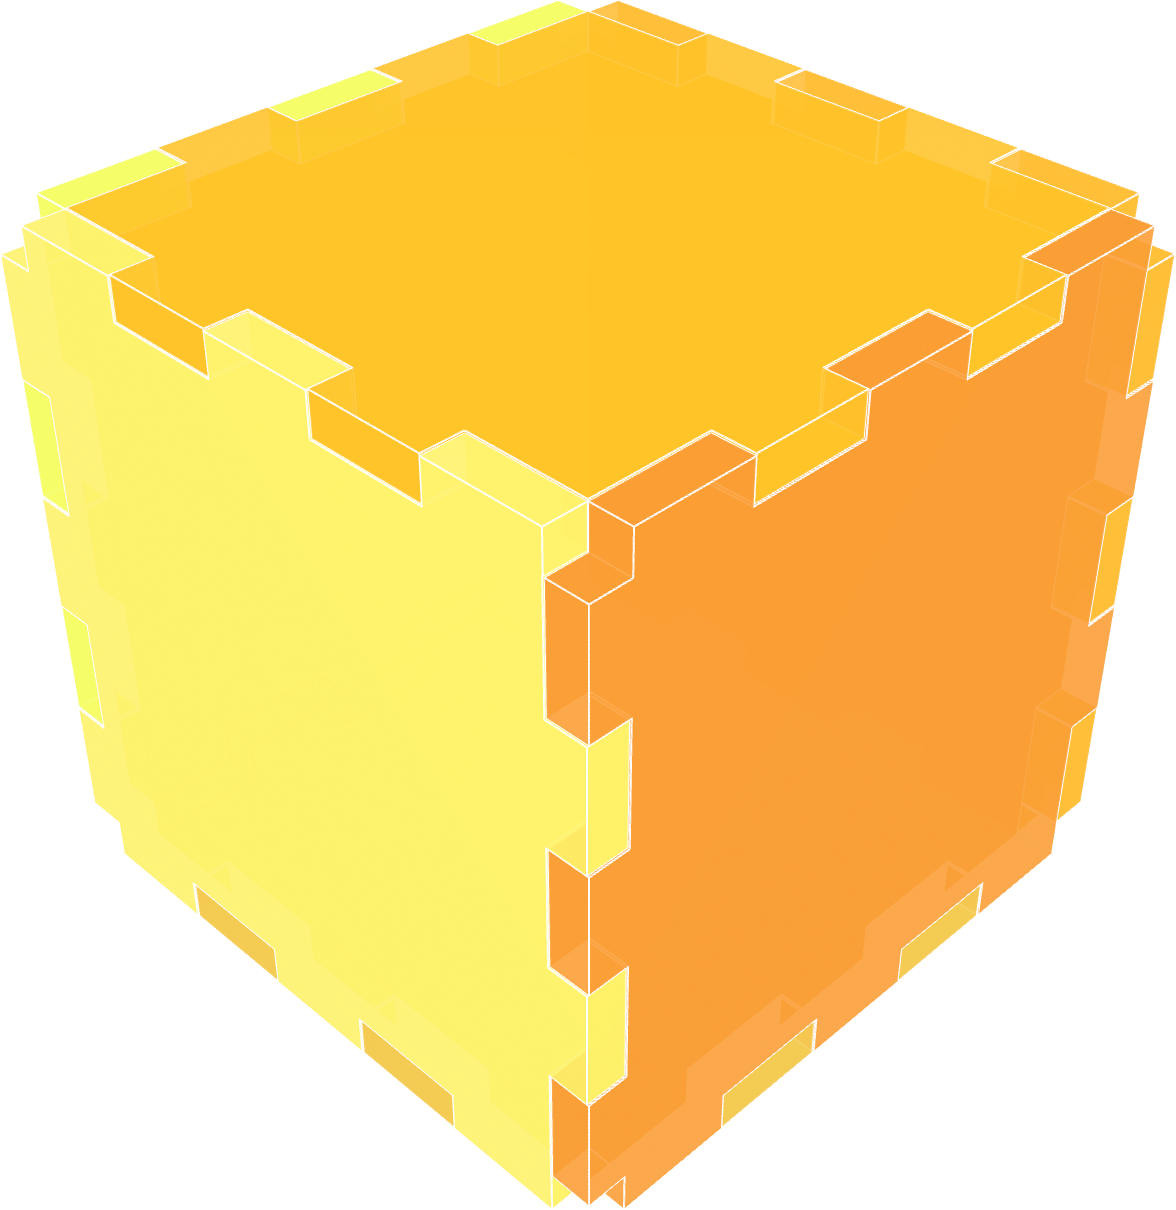
\includegraphics[width=\textwidth]{03-architecture-box-fingers}
    \caption{A box with finger joints.}
    \label{fig:corrupt:fingers}
  \end{subfigure}
  \caption{Modifications to shallow copies of the data
    corrupt the visualizations.}
  \label{fig:corrupt}
\end{figure}

We create deep copies of the data structures, to persist the
data of the snapshots. A deep copy of a data structure, is a
clone of all fields of that data structure. That means if a
data structure references dynamically allocated memory, we
do not clone the reference of the allocated memory to the
copy of the data structure. Instead, we allocate new memory
and duplicate the data to the newly allocated memory. Thus,
we make sure modifications on the copy do not alter the
original. Listing~\ref{lst:deep-copy} shows the effects of a
deep copy.

\begin{listing}[h]
\begin{minted}[
linenos
]{coffeescript}
data = createDynamicMemoryWith('foo')
copy = data.copy()

# both structures have the same copied data
data.dynamicMemory # = foo
copy.dynamicMemory # = foo

# alter the dynamically allocated memory
changeFooToBar(copy.dynamicMemory)

# a shallow copy will effect both,
# the data and the copy
copy.dynamicMemory # = bar
data.dynamicMemory # = bar

# a deep copy prevents this effect
data = createDynamicMemoryWith('foo')
deepCopy = data.deepCopy()

data.dynamicMemory # = foo
copy.dynamicMemory # = foo

changeFooToBar(copy.dynamicMemory)

copy.dynamicMemory # = bar
data.dynamicMemory # = foo
\end{minted}
\caption{A {\coffeescript} example showing the effects of a deep copy
  of data.}
\label{lst:deep-copy}
\end{listing}

% - needs-figure, needs-ref :: Immutable PipelineState
% allows timetravel visual debugging

The data that is passed between the \class{PipelineSteps} is
encapsulated in a \class{PipelineState}. The
\class{PipelineState} contains all data structures that are
ever to be computed by all \class{PipelineSteps}. It is
essentially a container for every computation result.

A snapshot is obtained by cloning the \class{PipelineState}
after the execution of a \class{PipelineStep}. The
\class{PipelineState} is an clonable data structure. A
cloneable data structure can be copied. We provide a deep
copy for the \class{PipelineState}, so that any changes to
the copy will not affect the original and vice-versa.
Figure~\ref{} \note{steps and snapshots flow} illustrates
how snapshots are obtained between two
\class{PipelineSteps}. The encapsulated data in the state
can be hierarchical and complex. We provide a fully
cloneable data structure. That means, any nested data
structure in the \class{PipelineState} implements a
cloneable interface and supports deep copies. Thus, we
ensure that modifications to any nested data by latter
\class{PipelineSteps} do not modify previous copies of the
data.


% \item Pipeline Implementation

%   \begin{enumerate}
%   \item the pipeline works as follows...
%     \begin{itemize}
%     \item Pipeline class
%     \item pipe interface for Step factories (compare listing above, stacked method)
%     \item create state factory -> use composition to persist intermediate results
%       (state is later accessed by node visualizer)
%     \item reduce approach -> pipe last state into next step to produce new state
%     \item show a listing of pseudo code, explaining how the pipeline works
%     \item benchmarking (measure time for intermediate steps vs whole processing)
%     \end{itemize}

%   \item it can be reused (because pipelining is a generic concept)
%     \begin{itemize}
%     \item classifier graph (classification method)
%     \item isolated testing (injectable pipeline)
%     \end{itemize}
%   \end{enumerate}

% \end{enumerate}


\subsection{The Client Package Connects All Features Into an
  Application}
\label{sec:client-to-application}
\note{concrete heading: platener instead of application}

% - Subsection overview

This section describes the code packages of {\platener}.
Furthermore, we explain the how {\convertify} is used by
{\platener} and how the user interface is connected to the
\class{Plugins}.

%     - needs-figure :: Application is separated into
%     Packages


\begin{figure}
  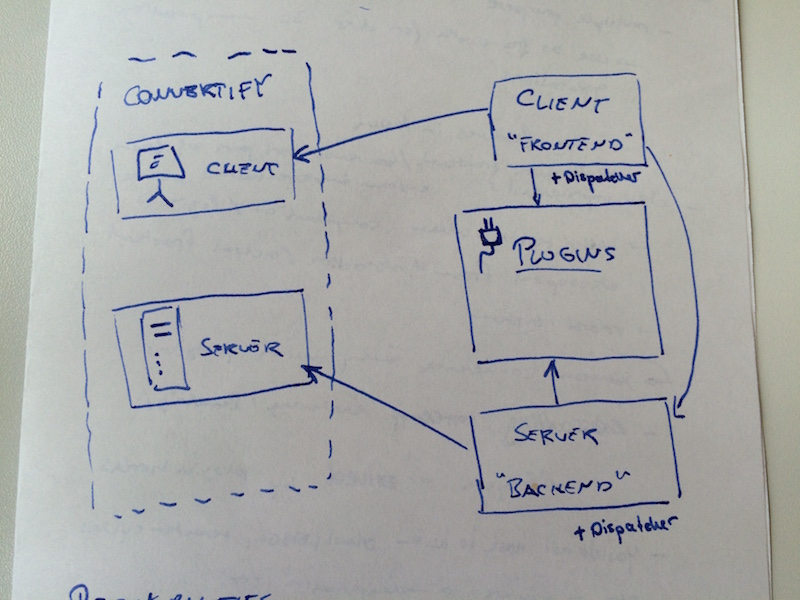
\includegraphics[width=1\columnwidth]{03-architecture_overview_current}
  \caption{Main Packages of the Platener Architecture}
  \label{fig:architectureOverviewCurrent}
\end{figure}

{\platener} is divided into the code packages {\convertify},
\name{Plugins} and \name{Client}.
Figure~\ref{fig:architectureOverviewCurrent} shows the
package diagram. Each package takes over a set of distinct
responsibilities.

\note{too generic here?}

The {\convertify} package is a framework, providing a
rendering engine and plugin management. The \name{Plugins}
package provides an exchangeable set of features for the
WebGL scene. The \name{Client} package gives the look and
feel of {\platener}. This package contains frontend
components, which make up the {\userinterface}. Also, a
\class{Dispatcher} is implemented in this package,
configuring the communication of plugins.

\note{text is missing here}

%     - needs-figure :: Client code connects all plugin
%     features with a user interface

%     - Use Framework to wire up everything, but not part of the
%       framework (Bundle and Protocols come in handy, Client code
%       implements a Dispatcher instance = the mediator)

%     - We have a WebApp and a Server package, which are both Client
%       code, because we have two types of applications
%     - the WebApp is an online service deployed for use by Makers
%     - the CLI tool is a service for batch processing or integration
%       with other applications

% **** The WebApp Package Builds a Cross-platform Web Page

%      - Subsubsection overview
%      - needs-ref :: Web Interfaces are built with HTML and CSS
%      - needs-ref :: The React library | copy from AOP paper
%      - needs-ref, needs-figure :: The Redux library (Dump Components and Smart Containers)
%      - needs-figure :: Using Redux dispatch in the Dispatcher
%      - Subsubsection summary

% **** The Server Package Allows Headless Batch Processing of Models

%      - Subsubsection overview
%      - A CLI tool runs in nodejs
%      - needs-ref :: Processing objects without opening a browser (isomorphic code)
%      - Processing multiple objects in sequence
%      - Integration with tools to be built in future
%      - Subsubsection summary


% \subsection{Package Responsibilities}

%  ensuring decoupled
% components. Thus a flexible, maintainable system is created.

% \emph{Convertify} provides generic tools which support plugins in manipulating
% {\threedmodel}s. This includes utilities for vector analysis as well as
% rendering routines and scene management. The application lifecycle can be
% initiated and observed via a \emph{Bundle}. A Bundle represents an instance of
% the application's computation unit. The Client and Server packages run a Bundle.

% \emph{Plugins} provide an exchangeable set of features which are used by the
% Client and Server package. A Plugin interacts with the Scene and its
% {\threedmodel}s via lifecycle events. E.g. a concrete conversion strategy
% provided by Platener is implemented by a single Plugin. Plugin features can be
% enabled for Client, Server or both.

% The \emph{Client} package gives the look and feel of the application. This
% package contains frontend components. The developer can choose any template
% engine\footnote{\url{http://www.sitepoint.com/overview-javascript-templating-engines/}}
% which serves the application's purpose. So the Client wires up the
% {\userinterface} and the computation logic.

% The \emph{Server} package is the headless\footnote{A headless web-application
%   runs without the graphical user interface of browsers.} counterpart to the
% Client package. A Command Line Interface enables the user to run the application
% without a browser. The Server also satisfies requests from the Client, such as
% caching and loading models in a RESTful
% interaction\footnote{\url{http://www.drdobbs.com/web-development/restful-web-services-a-tutorial/240169069}}.

% % \begin{itemize}
% % \item convertify: generic tools, helpers for 3d rendering, scene management,
% %   model manipulation, platener independent
% % \item client: look and feel, ux user interactions, wiring up/ firing up
% %   computations, implemented for platener
% % \item server: model storage/ cache, REST interaction, headless version of
% %   client, CLI-tool chain, implemented for platener
% % \item plugins: conversion specific computation and logic units, addons for
% %   frontend and backend, platener independent
% % \end{itemize}


% \subsection{Decoupling the Software into Packages}

% Decoupling the software into packages builds a robust system. Computation logic
% and UX components are kept apart, which allows isolated testing.

% \subsubsection{Dispatcher and Bundle on Client and Server}

% \myNotes{maybe put this up, so we understand earlier what the ClientDispatcher
%   is}

% The Server and Client package handle lifecycle events differently and use
% different protocols. That is because the Client package has to handle rendering
% and user interaction. The Server package merely computes the manipulated models
% and is used for batch processing of {\threedmodel}s. Therefore, we need two
% Dispatcher implementations for the client and for the server.

% A Bundle is the entry point for any client or server code. As the name
% indicates, a Bundle bundles all application code into a single instance. It
% references the specific \emph{ClientDispatcher} or \emph{ServerDispatcher},
% which are implemented in the Client or Server package respectively. Thus we can
% control the system by invoking protocol interfaces. The ClientBundle is exposed
% to the Client package. The ServerBundle is exposed to the ServerPackage.

% \section{Client Package}
% % ************************************************

% \subsection{Overview - Custom Frontend Code}

% \begin{itemize}
% \item when convertify framework, client is freespace to evolve yaself
% \item look and feel of the application
% \item task: connect logic to ui (speak with dispatcher) and build ui
% \item free choice of frontend framework (we take redux + react), but nothing
%   against jquery or angular or backbone or ...
% \item e.g. laser origami or brickify would choose a completely different
%   implementation of client -> custom per application
% \item react by facebook, redux by dan abramov, like flux architecure -> uni
%   directional dataflow, explicit state changes, data driven -> reduce side
%   effects and be efficient in coding and trace down errors easily
% \item \myNotes{diagram which shows benefits of flux architecture vs no flux
%     arch, look at intro vids for redux from dan abramov}
% \end{itemize}

% \subsection{React Templates}

% \begin{itemize}
% \item show html tree graph and how data communication goes wild when talking
%   with siblings
% \item ideally dumb components (dont know where data is coming from, just display
%   it)
% \item stateless, components directory
% \item WIP: before no redux, so there are some mixed up components left :S
% \item show short example how a dump component looks like, \myNotes{listing!}
% \end{itemize}

% \subsection{Redux Data-driven Control Flow}

% \begin{enumerate}
% \item Redux `dispatch` and state
%   \begin{itemize}
%   \item one state container
%   \item functional, no side effects
%   \item maybe copy or reference redux description (just explain why its awesome)
%   \item injected into react via context
%   \end{itemize}

% \item Smart Containers
%   \begin{itemize}
%   \item connect to state
%   \item containers know where data is from (vs dump components)
%   \item fitler and preprocess raw data, setup interaction events to trigger
%     actions
%   \item give data and callbacks to a component (they setup the actual ui, but
%     contain no visible elements themselves)
%   \item \myNotes{listing show how to connect and use component from other
%       listing}
%   \end{itemize}

% \item Manage Async Plugin Hell
%   \begin{itemize}
%   \item as described before, plugin data is not available on load
%   \item we can use Dispatcher and redux dispatch combined
%   \item protocols -> state change in plugins -> dispatch -> state change in
%     frontend
%   \item no polling or observing of data, fully reactive (system -> client communication)
%   \item as client has access to bundle, we can call interfaces exposed by
%     protocols (client -> system communication)
%   \end{itemize}
% \end{enumerate}

% \section{Server Package}
% % ************************************************

% \subsection{Overview - Custom Server Code}

% \begin{itemize}
% \item like client, can have custom implementations
% \item we have caching and cli (headless version of application)
% \item requires isomorphic code: execute on client and server equally
% \item \myNotes{isomorphic means...}
% \item threejs, polyfills, \myNotes{...}
% \end{itemize}

% \subsection{Model Cache}

% \begin{itemize}
% \item idea: build up repository of models when users interact with it
% \item taken from brickify: uploading meshlib version of model
% \end{itemize}

% \subsection{Test Pipeline}

% \begin{enumerate}
% \item WHY do we have a Test Pipeline?
%   \begin{itemize}
%   \item robustness tests
%   \item batch processing
%   \item headless version for integration with other projects
%   \item failure detection because of diversity of objects
%   \end{itemize}

% \item Headless Conversion of Objects
%   \begin{itemize}
%   \item run solutionselection plugin also
%   \item but dispatcher is setup a bit differently
%   \item no recomputation, no grid, no visualizer
%   \item scene manager will not render anything (unless, WIP we exchange webgl
%     rendering with headlessgl to produce screenshots of each conversion)
%   \item cli tool -> safe results into directories
%   \end{itemize}

% \item Reports
%   \begin{itemize}
%   \item = extended console logs
%   \item show how conversion was going
%   \item display failures, status, progress
%   \item in the end: sum up + give stats
%   \item WIP: current problems: not all conversions are garbage collected
%     correctly, will run out of memory after some conversions -.- (maybe nobody
%     has to know about that)
%   \end{itemize}

% \item Benchmarks
%   \begin{itemize}
%   \item xxx testmodels
%   \item we proposed mostly stacked as the best solution
%   \item too many arbitrary forms hindered plate conversion
%   \item just shows conversion stats (maybe all models vs box category only)
%   \item \myNotes{measure times for conversions and evaluate}
%   \end{itemize}
% \end{enumerate}

\end{document}
